\documentclass[aspectratio=169]{beamer}

\usepackage{graphicx}
\usepackage{import}
\usepackage{media9}
\usepackage{multimedia}
\usepackage{tikz}
\usetikzlibrary{backgrounds}
% \usetikzlibrary{external}
\usetikzlibrary{matrix}
\usetikzlibrary{positioning}
\usetikzlibrary{scopes} % brilliant library!

% \tikzexternalize

\pgfdeclarelayer{background}
\pgfdeclarelayer{foreground}
\pgfsetlayers{background,main,foreground}


\usetheme{Janelia}

\title[Janelia Theme]{The Metamorphosis of BigCAT --- Toward Streamlined Proofreading}
\subtitle{Toward Streamlined Proofreading}
% \subtitle{A custom modern minimalist Beamer theme designed from scratch}
\author{Philipp Hanslovsky}
\date{February 18, 2018}

\setcounter{showSlideNumbers}{1}

\begin{document}

\setcounter{showProgressBar}{0}
\setcounter{showSlideNumbers}{0}

\frame{\titlepage}

\begin{frame}
    \frametitle{Circuit Reconstruction}
    
    \begin{itemize}
          \item Dense reconstruction in EM data
          \item Connectivity graph
          \item Avoid critical errors
    \end{itemize}
\end{frame}

\begin{frame}
    \frametitle{Circuit Reconstruction}
    \begin{itemize}
          \item Machine Learning Algorithms
          \item Neuron boundary prediction
          \item Agglomeration
          \item Proof Reading
    \end{itemize}
\end{frame}

\begin{frame}
    \frametitle{BigCAT -- Yay!}
    \begin{itemize}
          \item Arbitrary Re-Slicing
          \item Painting (!!)
          \item Agglomeration
          \item Annotations
          \item Potential for heavy workload tasks on client
    \end{itemize}
\end{frame}

\begin{frame}
    \frametitle{BigCAT -- Nay!}
    \begin{itemize}
          \item No Ortho views
          \item Painting not multi-resolution
          \item No 3D
          \item Limited to a very specific use case
    \end{itemize}
\end{frame}

\begin{frame}
    \frametitle{BigCAT -- Want!}
    \begin{itemize}
          \item Ortho views with arbitrary reslicing
          \item 3D visualization of meshes (potentially generated on the fly)
          \item Multi-resolution painting
          \item (Guided) agglomeration with solver server
          \item Broadly applicable and extensible
    \end{itemize}
\end{frame} 

\begin{frame}
    \frametitle{Neuroglancer}
    \begin{itemize}
          \item Arbitrary Re-Slicing
          \item 3D mesh rendering
          \item Extensible
          \item No Painting
          \item No Neuron Mesh Generation for arbitrary data sets 
% (only for python in-memory volumes)
          \item Heavy number crunching on client side limited (memory and threading) \fbox{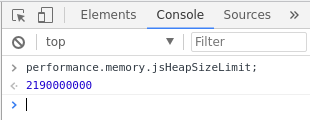
\includegraphics[width=4cm]{fig/chrome-heap-limit.png}}
          \item https://github.com/google/neuroglancer
% https://stackoverflow.com/a/23705446/1725687
% https://groups.google.com/a/chromium.org/forum/#!topic/chromium-dev/TUddM_rtgi4
    \end{itemize}
\end{frame}

\begin{frame}
    \frametitle{Agglomeration}
    \subimport{fig/}{agglomeration}
\end{frame}

\begin{frame}
    \frametitle{Agglomeration}
    \def\factor{1.0}
    \movie[%
    width=\factor\textwidth,%
    height=\factor\textheight,%
    ]{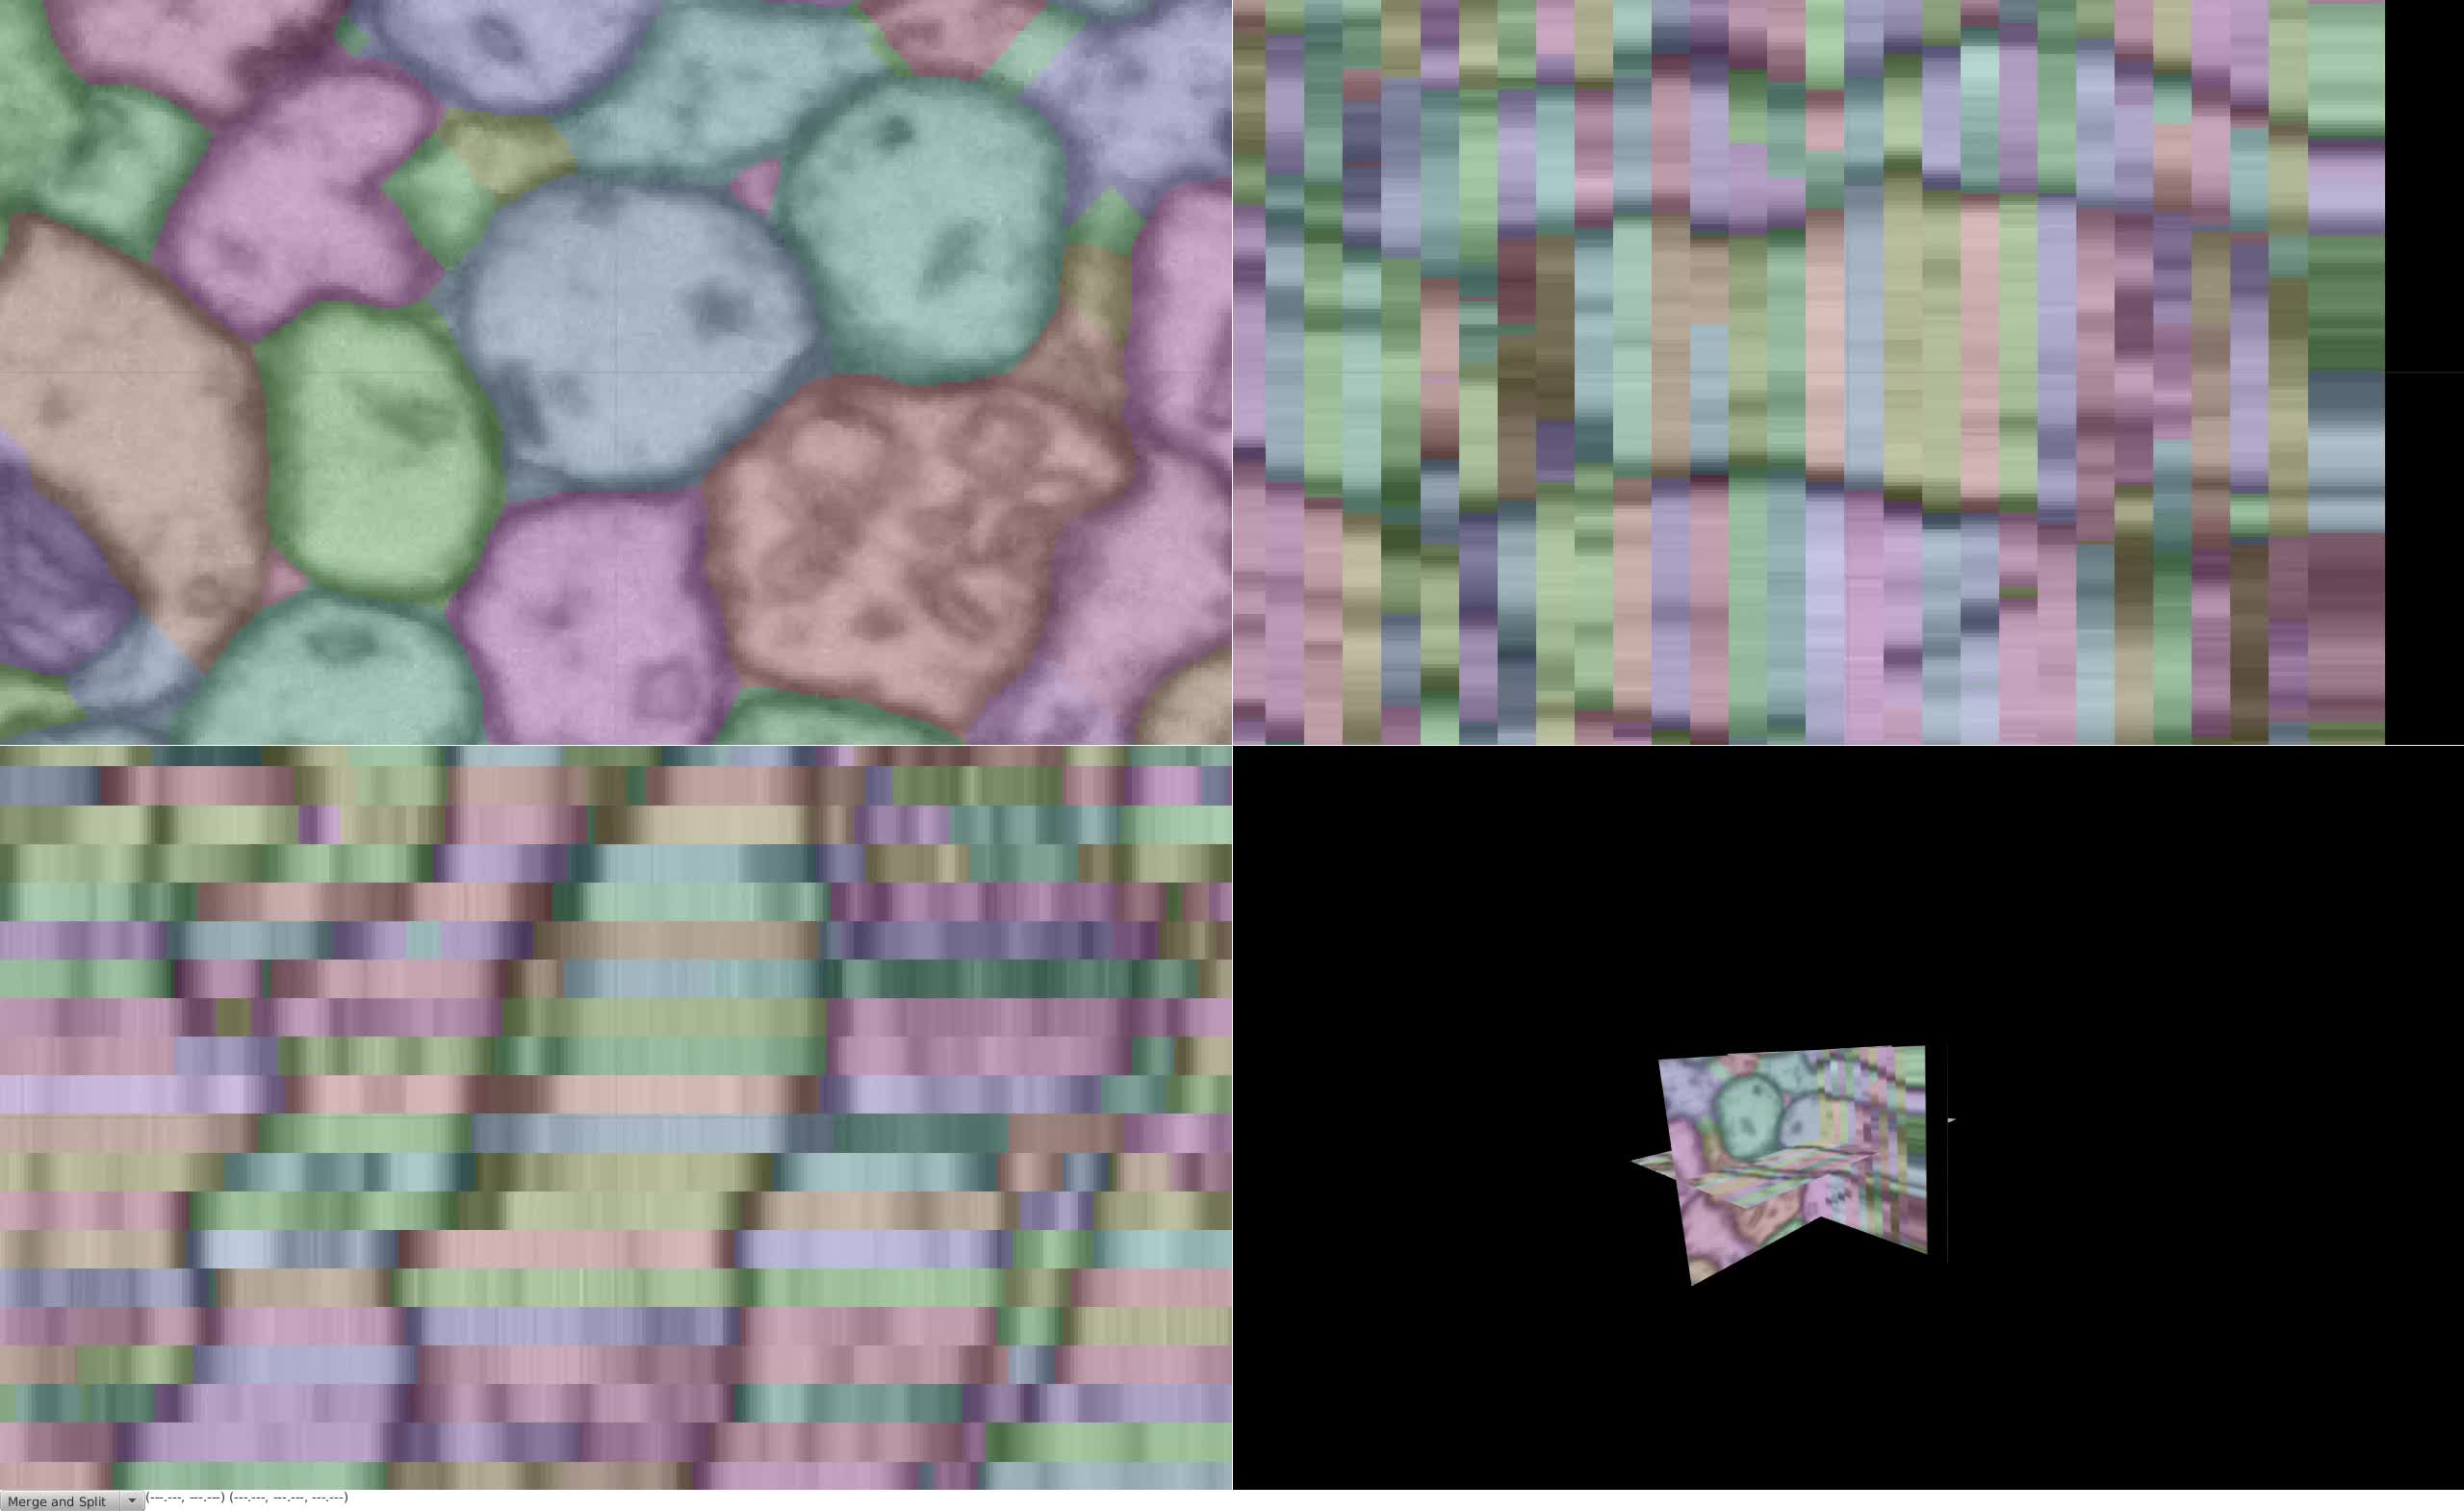
\includegraphics[width=\factor\textwidth]{vid/assignments-placeholder.jpg}}{vid/assignments.mp4}
    % show video
    % backend: c9ae08b
    % bigcat:  e84388e
    % start with fragment 2660 (blue)
\end{frame}

\begin{frame}
    \frametitle{Painting}
     \def\factor{1.0}
    \movie[%
    width=\factor\textwidth,%
    height=\factor\textheight,%
    ]{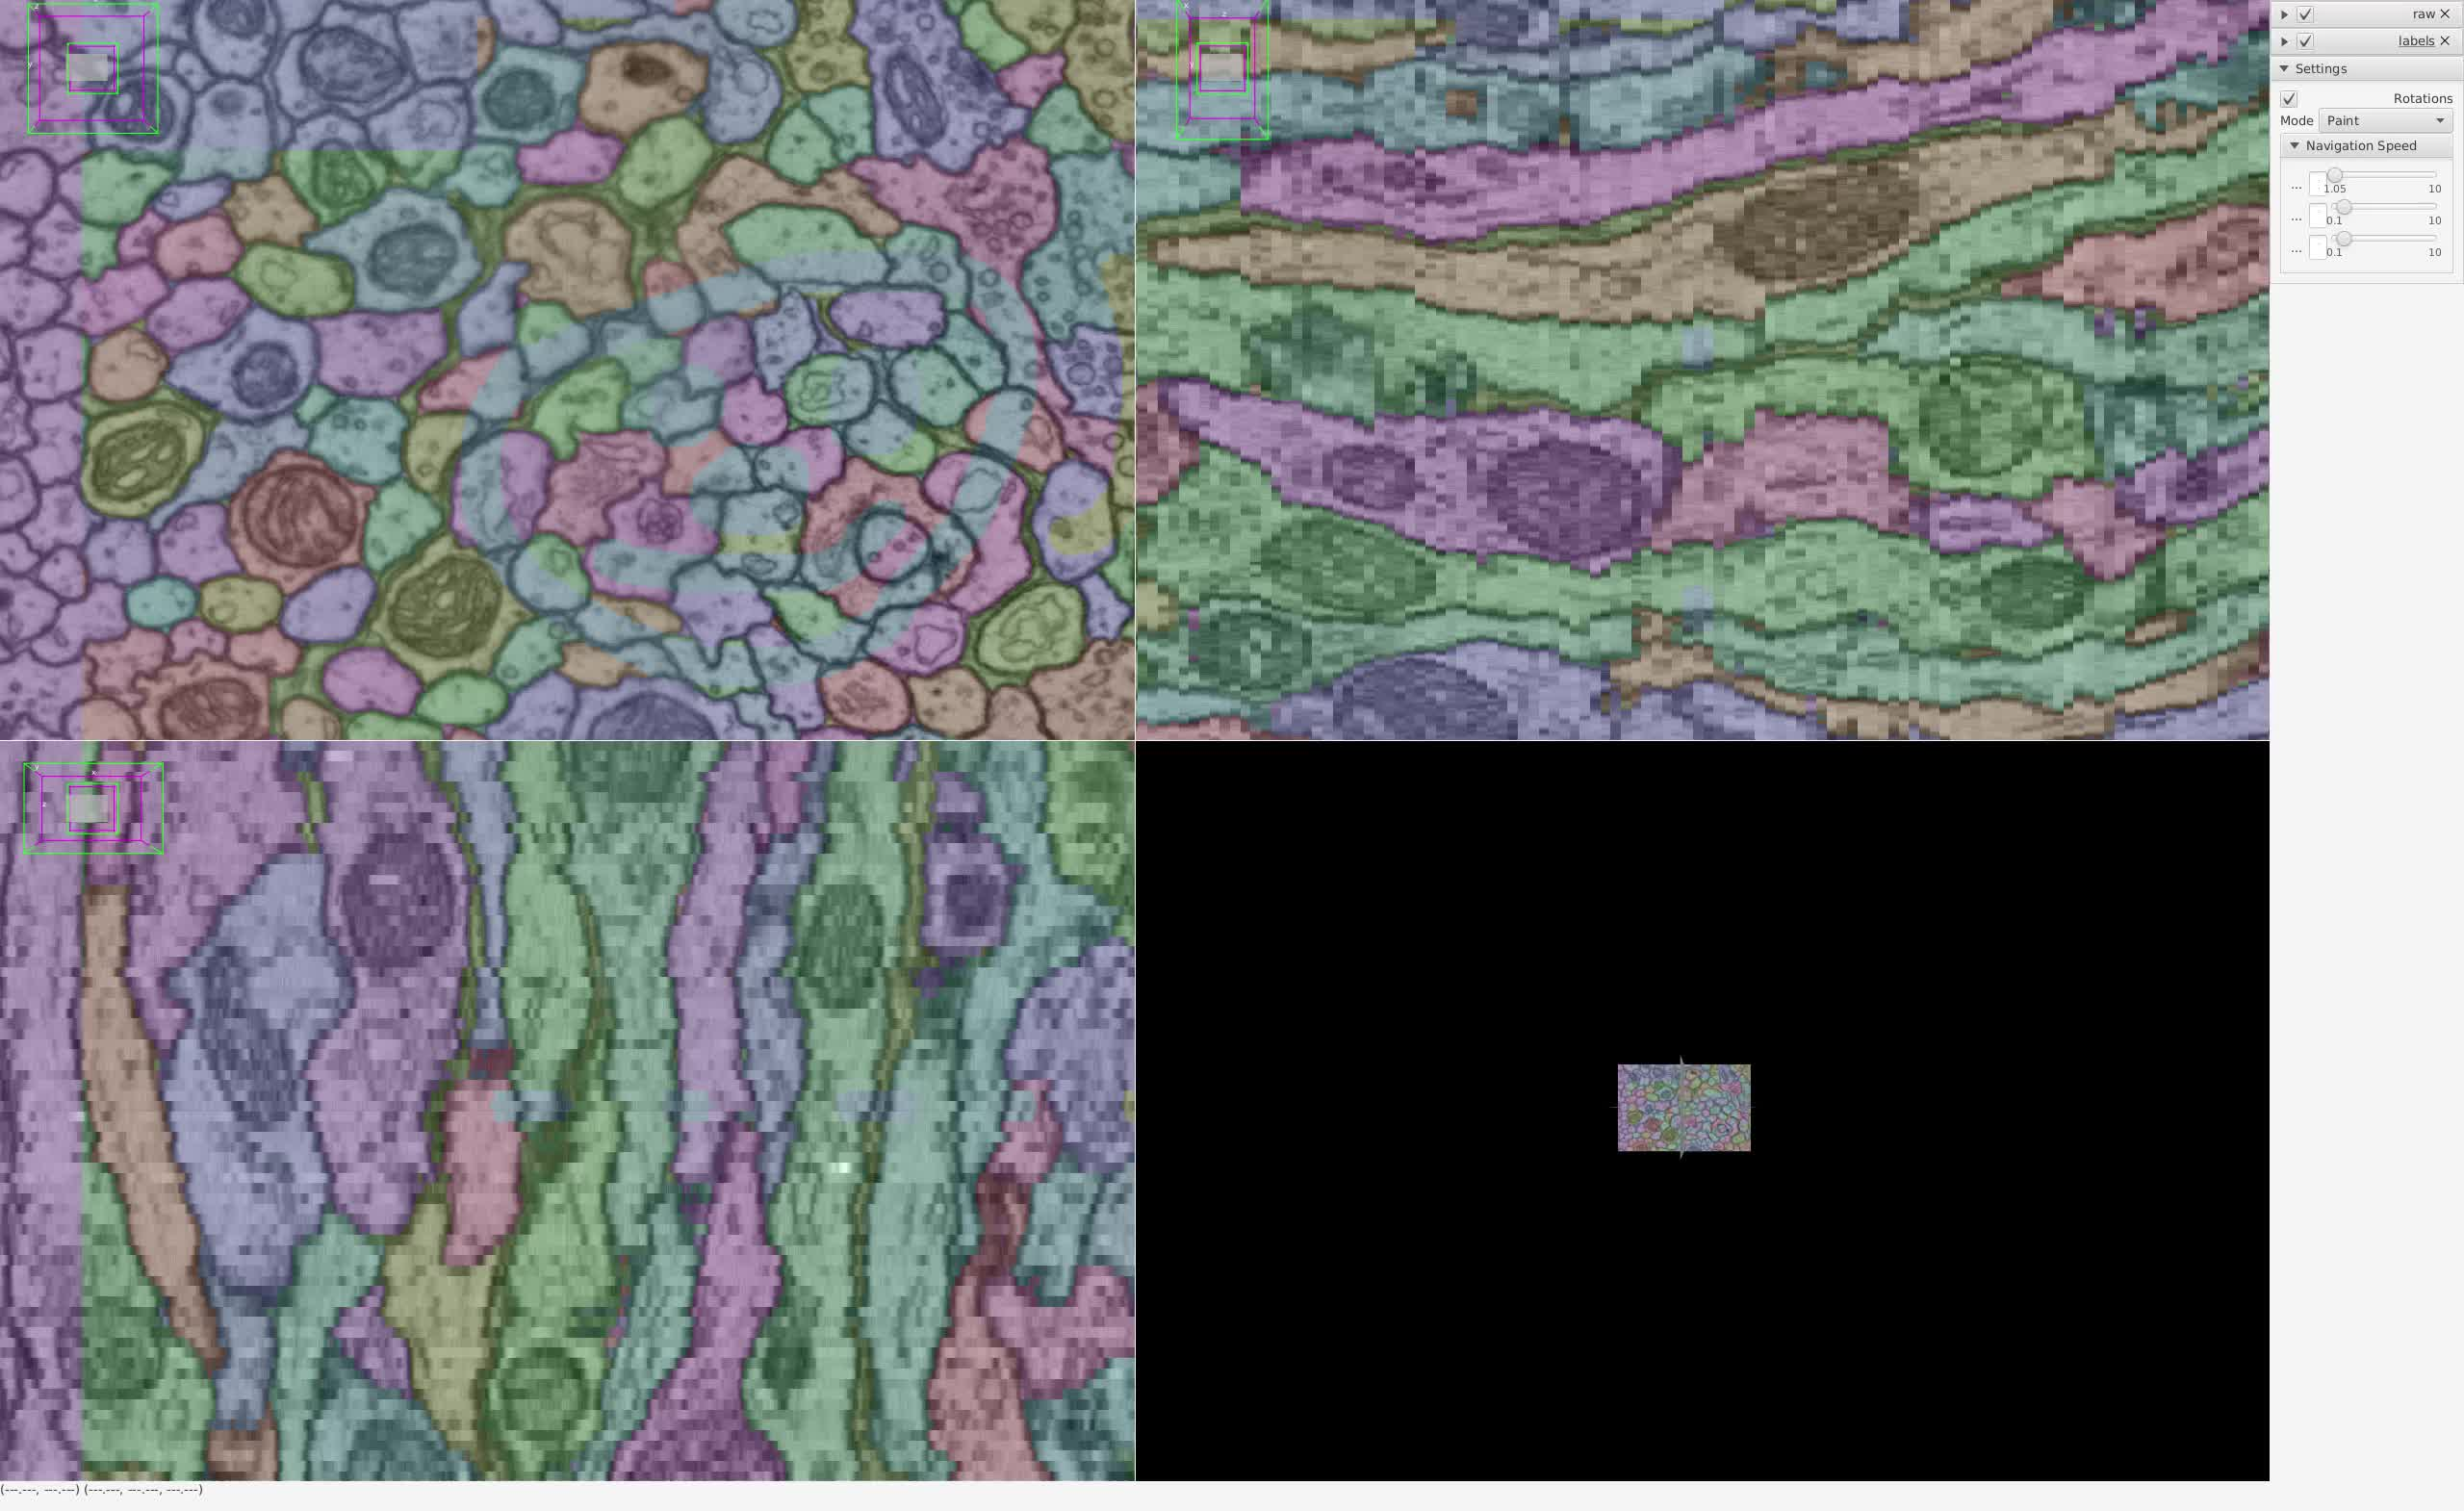
\includegraphics[width=\factor\textwidth]{vid/paint-placeholder.jpg}}{vid/paint.mp4}
\end{frame}

%     \def\colorOne{red}
%     \def\colorTwo{blue}
%     \def\colorThree{yellow}
%     \def\colorFour{green}
%     \def\colorFive{magenta}
%     \def\cellSize{1.4em}
% \begin{frame}
%     \frametitle{Painting}
%     \subimport{fig/}{paint}
% \end{frame}

% \begin{frame}
%     \frametitle{Painting}
%     \subimport{fig/}{paint-continued}
% \end{frame}

% \begin{frame}
%     \frametitle{Mesh Generation}
%     show video
% \end{frame}

% \begin{frame}
%     \frametitle{Mesh Generation}
%     \centering
%     \begin{tikzpicture}
%         \subimport{fig/}{mesh-cache}
%     \end{tikzpicture}
% \end{frame}



\end{document}


%%% Local Variables:
%%% mode: latex
%%% TeX-master: t
%%% End:
